\documentclass[11pt]{article}
%DIF LATEXDIFF DIFFERENCE FILE
%DIF DEL draft_old.tex   Fri Jul  7 17:12:46 2023
%DIF ADD draft_new.tex   Sun Jul  9 21:31:56 2023
	
%%%%%%%%%%%%%%%%%%%%%%%%%%%%%%%%%%%%%%%%%%%%%%%%%%%%%%%%%%%%%%%%%%%%%%
%\pdfminorversion=4
% NOTE: To produce blinded version, replace "0" with "1" below.
\newcommand{\blind}{0}

%%%%%%% IISE Transactions margin specifications %%%%%%%%%%%%%%%%%%%
% DON'T change margins - should be 1 inch all around.
\addtolength{\oddsidemargin}{-.5in}%
\addtolength{\evensidemargin}{-.5in}%
\addtolength{\textwidth}{1in}%
\addtolength{\textheight}{1.3in}%
\addtolength{\topmargin}{-.8in}%
\makeatletter
\renewcommand\section{\@startsection {section}{1}{\z@}%
                                   {-3.5ex \@plus -1ex \@minus -.2ex}%
                                   {2.3ex \@plus.2ex}%
                                   {\normalfont\fontfamily{phv}\fontsize{16}{19}\bfseries}}
\renewcommand\subsection{\@startsection{subsection}{2}{\z@}%
                                     {-3.25ex\@plus -1ex \@minus -.2ex}%
                                     {1.5ex \@plus .2ex}%
                                     {\normalfont\fontfamily{phv}\fontsize{14}{17}\bfseries}}
\renewcommand\subsubsection{\@startsection{subsubsection}{3}{\z@}%
                                    {-3.25ex\@plus -1ex \@minus -.2ex}%
                                     {1.5ex \@plus .2ex}%
                                     {\normalfont\normalsize\fontfamily{phv}\fontsize{14}{17}\selectfont}}
\makeatother
%%%%%%%%%%%%%%%%%%%%%%%%%%%%%%%%%%%%%%%%%%%%%%%%%%%%%%%%%%%%%%%%%%%%%%%%%

%%%%% IISE Transactions package list %%%%%%%%%%%%%%%%%%%%%%%%%%%%%%%%%%%%%%
\usepackage{amsmath}
\usepackage{amsfonts}
\usepackage{mathtools}
\usepackage{graphicx}
\usepackage{enumerate}
\usepackage{natbib} %comment out if you do not have the package
\usepackage{url} % not crucial - just used below for the URL
%%%%%%%%%%%%%%%%%%%%%%%%%%%%%%%%%%%%%%%%%%%%%%%%%%%%%%%%%%%%%%%%%%%%%%%

%%%%% Author package list and commands %%%%%%%%%%%%%%%%%%%%%%%%%%%%%%%%%%%%%%%%%%%%%
%%%%% Here are some examples %%%%%%%%%%%%%%
%	\usepackage{amsfonts, amsthm, latexsym, amssymb}
%	\usepackage{lineno}
%	\newcommand{\mb}{\mathbf}
%%%%%%%%%%%%%%%%%%%%%%%%%%%%%%%%%%%%%%%%%%%%%%%%%%%%%%%%%%%%%%%%%%%%%%%%%%%%%%
%DIF < 
%DIF PREAMBLE EXTENSION ADDED BY LATEXDIFF
%DIF UNDERLINE PREAMBLE %DIF PREAMBLE
\RequirePackage[normalem]{ulem} %DIF PREAMBLE
\RequirePackage{color}\definecolor{RED}{rgb}{1,0,0}\definecolor{BLUE}{rgb}{0,0,1} %DIF PREAMBLE
\providecommand{\DIFadd}[1]{{\protect\color{blue}\uwave{#1}}} %DIF PREAMBLE
\providecommand{\DIFdel}[1]{{\protect\color{red}\sout{#1}}}                      %DIF PREAMBLE
%DIF SAFE PREAMBLE %DIF PREAMBLE
\providecommand{\DIFaddbegin}{} %DIF PREAMBLE
\providecommand{\DIFaddend}{} %DIF PREAMBLE
\providecommand{\DIFdelbegin}{} %DIF PREAMBLE
\providecommand{\DIFdelend}{} %DIF PREAMBLE
\providecommand{\DIFmodbegin}{} %DIF PREAMBLE
\providecommand{\DIFmodend}{} %DIF PREAMBLE
%DIF FLOATSAFE PREAMBLE %DIF PREAMBLE
\providecommand{\DIFaddFL}[1]{\DIFadd{#1}} %DIF PREAMBLE
\providecommand{\DIFdelFL}[1]{\DIFdel{#1}} %DIF PREAMBLE
\providecommand{\DIFaddbeginFL}{} %DIF PREAMBLE
\providecommand{\DIFaddendFL}{} %DIF PREAMBLE
\providecommand{\DIFdelbeginFL}{} %DIF PREAMBLE
\providecommand{\DIFdelendFL}{} %DIF PREAMBLE
\newcommand{\DIFscaledelfig}{0.5}
%DIF HIGHLIGHTGRAPHICS PREAMBLE %DIF PREAMBLE
\RequirePackage{settobox} %DIF PREAMBLE
\RequirePackage{letltxmacro} %DIF PREAMBLE
\newsavebox{\DIFdelgraphicsbox} %DIF PREAMBLE
\newlength{\DIFdelgraphicswidth} %DIF PREAMBLE
\newlength{\DIFdelgraphicsheight} %DIF PREAMBLE
% store original definition of \includegraphics %DIF PREAMBLE
\LetLtxMacro{\DIFOincludegraphics}{\includegraphics} %DIF PREAMBLE
\newcommand{\DIFaddincludegraphics}[2][]{{\color{blue}\fbox{\DIFOincludegraphics[#1]{#2}}}} %DIF PREAMBLE
\newcommand{\DIFdelincludegraphics}[2][]{% %DIF PREAMBLE
\sbox{\DIFdelgraphicsbox}{\DIFOincludegraphics[#1]{#2}}% %DIF PREAMBLE
\settoboxwidth{\DIFdelgraphicswidth}{\DIFdelgraphicsbox} %DIF PREAMBLE
\settoboxtotalheight{\DIFdelgraphicsheight}{\DIFdelgraphicsbox} %DIF PREAMBLE
\scalebox{\DIFscaledelfig}{% %DIF PREAMBLE
\parbox[b]{\DIFdelgraphicswidth}{\usebox{\DIFdelgraphicsbox}\\[-\baselineskip] \rule{\DIFdelgraphicswidth}{0em}}\llap{\resizebox{\DIFdelgraphicswidth}{\DIFdelgraphicsheight}{% %DIF PREAMBLE
\setlength{\unitlength}{\DIFdelgraphicswidth}% %DIF PREAMBLE
\begin{picture}(1,1)% %DIF PREAMBLE
\thicklines\linethickness{2pt} %DIF PREAMBLE
{\color[rgb]{1,0,0}\put(0,0){\framebox(1,1){}}}% %DIF PREAMBLE
{\color[rgb]{1,0,0}\put(0,0){\line( 1,1){1}}}% %DIF PREAMBLE
{\color[rgb]{1,0,0}\put(0,1){\line(1,-1){1}}}% %DIF PREAMBLE
\end{picture}% %DIF PREAMBLE
}\hspace*{3pt}}} %DIF PREAMBLE
} %DIF PREAMBLE
\LetLtxMacro{\DIFOaddbegin}{\DIFaddbegin} %DIF PREAMBLE
\LetLtxMacro{\DIFOaddend}{\DIFaddend} %DIF PREAMBLE
\LetLtxMacro{\DIFOdelbegin}{\DIFdelbegin} %DIF PREAMBLE
\LetLtxMacro{\DIFOdelend}{\DIFdelend} %DIF PREAMBLE
\DeclareRobustCommand{\DIFaddbegin}{\DIFOaddbegin \let\includegraphics\DIFaddincludegraphics} %DIF PREAMBLE
\DeclareRobustCommand{\DIFaddend}{\DIFOaddend \let\includegraphics\DIFOincludegraphics} %DIF PREAMBLE
\DeclareRobustCommand{\DIFdelbegin}{\DIFOdelbegin \let\includegraphics\DIFdelincludegraphics} %DIF PREAMBLE
\DeclareRobustCommand{\DIFdelend}{\DIFOaddend \let\includegraphics\DIFOincludegraphics} %DIF PREAMBLE
\LetLtxMacro{\DIFOaddbeginFL}{\DIFaddbeginFL} %DIF PREAMBLE
\LetLtxMacro{\DIFOaddendFL}{\DIFaddendFL} %DIF PREAMBLE
\LetLtxMacro{\DIFOdelbeginFL}{\DIFdelbeginFL} %DIF PREAMBLE
\LetLtxMacro{\DIFOdelendFL}{\DIFdelendFL} %DIF PREAMBLE
\DeclareRobustCommand{\DIFaddbeginFL}{\DIFOaddbeginFL \let\includegraphics\DIFaddincludegraphics} %DIF PREAMBLE
\DeclareRobustCommand{\DIFaddendFL}{\DIFOaddendFL \let\includegraphics\DIFOincludegraphics} %DIF PREAMBLE
\DeclareRobustCommand{\DIFdelbeginFL}{\DIFOdelbeginFL \let\includegraphics\DIFdelincludegraphics} %DIF PREAMBLE
\DeclareRobustCommand{\DIFdelendFL}{\DIFOaddendFL \let\includegraphics\DIFOincludegraphics} %DIF PREAMBLE
%DIF END PREAMBLE EXTENSION ADDED BY LATEXDIFF

\begin{document}

		%%%%%%%%%%%%%%%%%%%%%%%%%%%%%%%%%%%%%%%%%%%%%%%%%%%%%%%%%%%%%%%%%%%%%%%%%%%%%%
	\def\spacingset#1{\renewcommand{\baselinestretch}%
		{#1}\small\normalsize} \spacingset{1}
	%%%%%%%%%%%%%%%%%%%%%%%%%%%%%%%%%%%%%%%%%%%%%%%%%%%%%%%%%%%%%%%%%%%%%%%%%%%%%%

	\if0\blind
	{
		\title{\bf Concurrent Data Assimilation for Model-guided Learning of Cardiac Potassium Channel Activities}
		\author{Author information is purposely removed for double-blind review}
		\date{}
		\maketitle
	} \fi

	\if1\blind
	{
        \title{\bf \emph{IISE Transactions} \LaTeX \ Template}
		\author{Author information is purposely removed for double-blind review}

\bigskip
		\bigskip
		\bigs   kip
		\begin{center}
			{\LARGE\bf \emph{IISE Transactions} \LaTeX \ Template}
		\end{center}
		\medskip
	} \fi
	\bigskip

\begin{abstract}
Potassium channels (K\textsubscript{v}) are responsible for repolarizing the action potential in cardiomyocytes. There is a variety of K\textsubscript{v} isoforms and corresponding currents (e.g., I\textsubscript{Kto}, I\textsubscript{Kslow1}, I\textsubscript{Kslow2}) that contribute to different phases of repolarization. Because only the sum of their activities can be measured in the form of currents (I\textsubscript{Ksum}), there is a need to decompose into individual K\textsuperscript{+} currents and their characteristics. Most existing studies separate and make inference of K\textsubscript{v} activities via curve-fitting procedures, but there are limitations such that: 1) curve-fitting decomposition only relies on the shape of K\textsuperscript{+} current traces, which does not discern the underlying kinetics and interactions; 2) I\textsubscript{Ksum} traces can only be fitted for one clamp voltage at each time, and estimated information is analyzed in a population-averaged way later. Here, we develop a novel concurrent data assimilation method that calibrates biophysics-based subject-specific computer models to decompose and delineate kinetics of K\textsubscript{v} isoforms with multiple voltage-clamp responses simultaneously. The proposed method is evaluated and validated with whole-cell I\textsubscript{Ksum} recordings from wild-type and chronically glycosylation-deficient cardiomyocytes. Experimental results show that the proposed method effectively handles multiple responses in the voltage-clamp protocol and describes the glycosylation-conferred perturbations observed experimentally to various K\textsubscript{v} isoforms. In addition, we develop a graphical-user-interface (GUI) application that provides an enabling tool to biomedical scientists. The proposed method and pertinent software are shown to have strong potential to study K\textsubscript{v} kinetics in various heart diseases.
\end{abstract}

\noindent%
{\it Keywords:} Data assimilation, in-silico modeling, model calibration, cardiac potassium channels, congenital disorders of glycosylation

%\newpage
\spacingset{1.5} % DON'T change the spacing!

\section{Introduction}
Potassium channels (K\textsubscript{v}) play critical roles in the electrical conduction system of the heart, particularly in the repolarization phase of the action potential (AP). The AP is a change of membrane potential over time, representing the net electrical activity in a cardiomyocyte, and the AP shape and duration are primarily determined by K\textsubscript{v} isoforms. The ability of the heart to pump blood through the body in an appropriate rhythm is controlled by electrical signaling. Hence, even modest changes in K\textsubscript{v} activities can significantly affect the AP duration and the QT interval, which lead to fatal heart diseases \citep{ravens2008role}. As shown in Figure~\ref{fig:ap_currents}, the different phases of AP repolarization in mouse cardiomyocytes are the result of the coordinated activity of a variety of K\textsubscript{v} isoforms (e.g., K\textsubscript{v}4.2, K\textsubscript{v}1.5, and K\textsubscript{v}2.1) and their corresponding currents (e.g., I\textsubscript{Kto}, I\textsubscript{Kslow1}, and I\textsubscript{Kslow2}). There are other major voltage-gated ion channels (VGICs), such as for Na\textsuperscript{+} (Na\textsubscript{v}) and Ca\textsuperscript{2+} (Ca\textsubscript{v}), that also contribute to the AP. The Na\textsubscript{v} are primarily responsible for the AP upstroke in the depolarization phase, while the Ca\textsubscript{v} control the cellular contraction. Aberrant activities of ion channels can significantly impact the AP and lead to fatal arrhythmias. Using whole-cell voltage-clamp recording methods, only the collective activities of K\textsubscript{v} isoforms can be measured reliably as the sum of all K\textsuperscript{+} currents (I\textsubscript{Ksum}), and these K\textsubscript{v} isoforms have overlapping biophysical properties (i.e., voltage dependence of gating and kinetics), which complicate the ability to separate one type of I\textsubscript{K} from another \citep{brouillette2004functional}. K\textsubscript{v} activities can be altered in various cardiomyopathies \citep{tristani2001molecular,giudicessi2012potassium}, thus there is an urgent need to decompose I\textsubscript{Ksum} more rigorously into individual K\textsuperscript{+} currents and estimate gating kinetics of K\textsubscript{v} isoforms to understand their pathological roles by comparing their activities in healthy versus diseased hearts and cardiomyocytes.
\begin{figure}[!ht]
    \centering
    \includegraphics{figs/ap_currents.pdf}
    \caption{(a) Ventricular action potential in mouse cardiomyocytes and (b) diverse K\textsubscript{v} isoforms and their currents contributing to the AP shape.}
    \label{fig:ap_currents}
\end{figure}

Transgenic mouse models are the most commonly used animal models that have provided insights into cardiac research despite the differences between rodents and humans; the isoforms expressed in both small and large mammals share many similarities \citep{milani2014small}. Most existing studies using mouse models separate individual K\textsuperscript{+} currents mathematically via a curve-fitting procedure \citep{costantini2005homeodomain,ednie2019reduced2,teng2022tmem65}, assuming the I\textsubscript{Ksum} current trace represents the summation of exponential decay functions (two or three, usually) and a constant term; each represents the shape of individual K\textsuperscript{+} currents. However, the ability to scrutinize the kinetics and dynamics of individual K\textsubscript{v} isoforms is limited by this traditional method because: 1) curve-fitting decomposition only relies on the shape of K\textsuperscript{+} current traces as discreet exponential functions which does not discern the underlying kinetics and interactions of K\textsubscript{v} isoforms; 2) I\textsubscript{Ksum} traces can only be decomposed for one clamp voltage at a time, and estimated information from each fitting is analyzed in a population-averaged way later. New methods are urgently needed to simultaneously delineate the underlying kinetics of multiple I\textsubscript{Ksum} traces from the same cell concurrently for a better understanding of K\textsubscript{v} channels and their roles as well as cellular variability in diseased cardiomyocytes.

This paper presents a new approach of subject-specific concurrent data assimilation for model-guided learning of K\textsubscript{v} isoforms. First, computer models of K\textsubscript{v} and their currents are designed with parameters that control the kinetic rates and, in turn, determine the currents. It is worth mentioning that K\textsuperscript{+} currents are generated based on the mathematically simulated gating mechanism. Second, we perform a sensitivity analysis of the kinetic parameters using fractional factorial designs to identify the parameters that have significant effects on the current generation. Several markers are defined that best represent the characteristics of the K\textsuperscript{+} currents in different perspectives. Third, a calibration routine is proposed to adjust parameters selected by the sensitivity analysis to couple \textit{in-silico} models with \textit{in-vitro} data of I\textsubscript{Ksum} recordings from the same cell concurrently. Last, low-dimensional embedding is utilized to visualize calibrated parameters in a collective way across the cells. The proposed methodology is evaluated and validated by comparing I\textsubscript{Ksum} recordings on healthy control versus chronically glycosylation-deficient cardiomyocyte. Glycosylation is a co/posttranslational modification that is critical for protein functions including activities of K\textsubscript{v} and other VGICs \citep{ohtsubo2006glycosylation,ednie2012modulation}. Our in-vitro experiments showed that chronic reduction in cardiomyocyte N-glycosylation modulates VGIC activities and contribute to both electrical and contractile dysfunction \citep{ednie2013sialicNav1,ednie2015sialicKv,ednie2019reduced}. In fact, these studies also showed that reduced cardiomyocyte complex N-glycosylation is sufficient to cause dilated cardiomyopathy (DCM), which is the third most common cause of heart failure and the major reason for heart transplantation \citep{weintraub2017dilated}.

Experimental results show that the proposed method provides reliable estimations of K\textsubscript{v} currents with underlying kinetics and successfully captures cellular variability. For example, it verifies the experimental data that showed the significant reduction in the current magnitude and elongated decaying for the glycosylation-deficient cardiomyocyte group. Additionally, computational modeling estimates channel kinetics, which was not possible in the electrophysiological experiments alone. Cellular variability is visualized by low-dimensional embedding of calibration parameters into 3D space, which shows one of the powers of systematic computer models that allow one to predict how changes in VGICs impact cellular functions. Further, we develop a graphical-user-interface (GUI) application to make the proposed method accessible to biomedical scientists for investigating K\textsubscript{v}-related channelopathy that is available as online supplemental material. The proposed method shows strong potential for modeling the kinetics and gating mechanism of K\textsubscript{v} to study heart diseases. Our contributions are summarized as follows:
\begin{itemize}
    \item We model the underlying kinetics of K\textsubscript{v} isoforms from I\textsubscript{Ksum} recordings, which enables to simulate individual K\textsuperscript{+} currents based on biophysical principles.
    \item We develop a subject-specific concurrent data assimilation routine that learns I\textsubscript{Ksum} recordings measured from the same cell at multiple membrane potentials simultaneously rather than a single I\textsubscript{Ksum} trace independently to model cellular-level dynamics.
    \item The prediction uncertainty is quantified and the distribution of kinetic parameters is visualized using low-dimensional embedding.
    \item A GUI application is provided to make the proposed method an enabling tool for biomedical scientists.
\end{itemize}
The software package of the GUI application, tutorial, and reproducible MATLAB codes for modeling and analysis results are available as supplementary material.

\section{Research Background}
\subsection{Data Assimilation and Calibration of Cardiac Models}
The functionality of the heart to pump blood through the body is controlled by electrical signals generated by the organ itself. Cardiac electrophysiology has contributed significantly to our understanding of the heart and disease-related modifications, such as congenital disorders of glycosylation (CDG). Advancements in laboratory techniques allow researchers to study molecular-level activities in cardiomyocytes via measuring ionic currents conducted through VGICs. For example, whole-cell current recordings are used to show the functions of a certain gene that encodes $\alpha$ subunits of Na\textsubscript{v} in human cardiomyocytes, leading to a small but inherent and chronic risk of acquired arrhythmia \citep{splawski2002variant}; pathophysiological roles of reduced sialylation impacting Na\textsubscript{v} and K\textsubscript{v} activities in mouse cardiomyocytes \citep{ednie2015sialicNav2,ednie2015sialicKv}; modulation of O-glycosylation causing aberrant K\textsubscript{v} activities \citep{schwetz2011sialic}. However, in-vitro experiments alone are limited to investigate detailed channel activities. There is a need to assimilate experimental data to estimate information that are not able to be observed directly. Traditionally, a curve-fitting method is used to make inferences, which assumes a functional form of information to estimate (e.g., individual currents of K\textsubscript{v} isoforms) \citep{liu2011dissection}.

In contrast, computer models consist of mathematical equations describing biophysical properties and physiological functions compatible with experimental observations. Mathematical and computational modeling allows for studying the heart in a quantitative and predictive way \citep{whittaker2020calibration}. Computer models, coupled with experimental observations, provide integrative insights into the data by calibrating model parameters \citep{winslow2011integrative}. For example, models can be used to interpolate processes not directly observed in experiments and extrapolate to novel conditions such as disease-related perturbations \citep{rodriguez2010systems}. From an engineering perspective, computer models of ion channels are dynamic system simulations that represent continuously changing gating kinetics. The dynamic nature of the models complicates the calibration process. Complex nonlinear structures of cardiac computer models also make calibration difficult. We developed statistical metamodeling and sequential design \citep{du2015statistical}, nonlinear optimization algorithms \citep{du2013silico,du2017silico}, and a heuristic optimization method \citep{kim2022simulation} in our previous in-silico studies to cope with the complexity of cardiac models. However, all these studies are based on current-shape parameters via curve fitting, or characteristic curves/statistics from additional curve fitting applied to estimated currents. In addition, only population-average models are derived and calibrated via learning the entire dataset for each healthy and diseased group. Little work has been done to leverage computer models to calibrate and delineate kinetic dynamics of K\textsubscript{v} isoforms with multiple voltage-clamp responses simultaneously.

\subsection{Congenital Disorders of Glycosylation}
Protein glycosylation is one of the most abundant and diverse forms of co/posttranslational modifications that impact essential protein functions, such as modulation of receptor or ion channel activities \citep{ohtsubo2006glycosylation,ednie2012modulation}. A growing number of studies have shown the association between altered glycosylation and heart diseases, such as dilated cardiomyopathy (DCM) and hypertrophic cardiomyopathy \citep{ednie2019reduced2,ohtsubo2006glycosylation}. It is reported that up to 20\% of patients with congenital disorders of glycosylation (CDG), who commonly show modest reductions in protein glycosylation, present with cardiac deficits, including idiopathic DCM \citep{marques2017cardiac}. However, uncovering the underlying pathological mechanisms still remains elusive. We have investigated how regulated glycosylation contributes to heart failure in the context of electrophysiology. Electrical signaling is orchestrated activities of a variety of ion channels and transporters. VGICs are heavily glycosylated, with ~30\% of the channel mass consisting of N-/O-linked glycans \citep{ednie2012modulation}. Glycosylation is a multi-step process and usually ends with sialic acid added. We reported that a saturating, electrostatic effect of negatively charged sialic attached to the terminal of N-/O-glycan branches significantly altered electrical signaling in Na\textsubscript{v} \citep{ednie2013sialicNav1,ednie2015sialicNav2} as well as K\textsubscript{v} \citep{ednie2015sialicKv}. Computational modeling has been used to further investigate the functional role of reduced sialylation in Na\textsubscript{v} and K\textsubscript{v} \citep{du2015statistical,du2017silico}.

\section{Research Methodology}
\subsection{Computer Models of Potassium Channel Isoforms}
Because of the relative ease at which their genetics can be altered, mice have been useful models for studying cardiac electric signaling \citep{milani2014small,nerbonne2004studying}. In ventricular and atrial mouse cardiomyocytes, there are three major components of I\textsubscript{Ksum}: rapidly inactivating transient outward K\textsuperscript{+} currents (I\textsubscript{Kto,f} and/or I\textsubscript{Kto,s}), which are conducted through K\textsubscript{v}4.2 and K\textsubscript{v}1.4 respectively, slowly inactivating delayed rectifier K\textsuperscript{+} currents (I\textsubscript{Kslow1} and I\textsubscript{Kslow2}), which are conducted through K\textsubscript{v}1.5/K\textsubscript{v}2.1, and the non-inactivating steady-state K\textsuperscript{+} current (I\textsubscript{Kss}) \citep{xu1999four}. I\textsubscript{Kto,s} (K\textsubscript{v}1.4) is primarily found in septal cardiomyocytes \citep{bondarenko2004computer}. In this study, we only include I\textsubscript{Kto,f} in I\textsubscript{Kto}, because our in-vitro studies focused on the ventricular apex myocytes. However, I\textsubscript{Kto} can be easily modified according to the region of ventricular cardiomyocytes. We model these four dominant K\textsuperscript{+} currents: I\textsubscript{Kto}, I\textsubscript{Kslow1}, I\textsubscript{Kslow2}, and I\textsubscript{Kss}. Figure~\ref{fig:kcurrent_example}(b) illustrates the shape of the primary K\textsuperscript{+} currents and their contribution to the whole-cell I\textsubscript{K} trace (I\textsubscript{Ksum}) given the protocol in Figure~\ref{fig:kcurrent_example}(a) that applies 0 mV voltage pulse from holding potential -70 mV from time $t^{(h)}$ to $t^{(e)}$. Figure~\ref{fig:kcurrent_example}(c) and (d) show a range of voltage steps from -30 mV to 50 mV in 10 mV increments and consequent changes in I\textsubscript{Ksum}. Because of their shape, I\textsubscript{Kss} is assumed as a constant and the other currents an exponential function in the traditional data-driven curve-fitting approach. In this approach, if all four current models are included, I\textsubscript{Ksum} is defined by \eqref{eq:expl_fitting} (i.e., tri-exponential fitting) with the shape parameters such as amplitude $\mathrm{A}_{i}$ and time constant $\tau_{i}$ for $i \in \{\mathrm{Kto}, \mathrm{Kslow1}, \mathrm{Kslow2}, \mathrm{Kss}\}$. In some cases, it is reduced to a bi-exponential function combining I\textsubscript{Kslow1} and I\textsubscript{Kslow2}. 
\begin{figure}[!ht]
    \centering
    \includegraphics{figs/kcurrent_example.pdf}
    \caption{Example of voltage-clamp protocol and K\textsuperscript{+} current traces. (a) Clamp-voltage pulse of 0 mV from the holding potential -70 mV. (b) Dominant K\textsuperscript{+} currents and their contributions to I\textsubscript{Ksum}. (c) Series of clamp-voltage pulses (-30-50 mV in 10 mV increments) from the holding potential -70 mV and (d) consequent I\textsubscript{Ksum} traces.}
    \label{fig:kcurrent_example}
\end{figure}
\begin{equation}
    \label{eq:expl_fitting}
    \mathrm{I}_{\mathrm{Ksum}} = \mathrm{A}_{\mathrm{Kto}}e^{-t/\tau_{\mathrm{Kto}}} + \mathrm{A}_{\mathrm{Kslow1}}e^{-t/\tau_{\mathrm{Kslow1}}} + \mathrm{A}_{\mathrm{Kslow2}}e^{-t/\tau_{\mathrm{Kslow2}}} +  \mathrm{A}_{\mathrm{Kss}}.   
\end{equation}

We developed mouse K\textsubscript{v} models based on \citep{bondarenko2014compartmentalized,asfaw2020compartmentalized}, using the Hodgkin-Huxley modeling scheme that has been used for various species, such as humans \citep{ten2004model} and rabbits \citep{mahajan2008rabbit}. This type of model consists of two gating variables controlling the channel conductance, and its canonical form is defined by \eqref{eq:hh_ex}
\begin{equation}
    \label{eq:hh_ex}
    \mathrm{I}_{\mathrm{K}} = G_{\mathrm{K}}a^{n}i^{m}(V-E_{\mathrm{K}}),
\end{equation}
where $G_{\mathrm{K}}$ is the maximum conductance, $a^{n}$ and $i^{m}$ are the gating variables for $n,m \in \mathbb{N}$, $V$ is the transmembrane potential, and $E_{\mathrm{K}}$ is the K\textsuperscript{+} Nernst potential. $V-E_{\mathrm{K}}$ implies the driving force of the ion movement. Important components in \eqref{eq:hh_ex} are the gating variables $a$ and $i$, representing the fraction of activation and recovery from inactivation of the channel where $a,i \in [0,1]$. These processes are governed by first-order kinetics and voltage-dependent transition rates $\alpha$ and $\beta$. $\alpha$ is the rate at which a gate in a closed state opens, whereas $\beta$ is the rate at which a gate in an open state closes. Equation~\eqref{eq:gv} shows a schematic relationship of this gating kinetics. $n$ and $m$ represent the numbers of activation and inactivation gates, which are dependent on a particular K\textsubscript{v} isoform and determined by specific kinetics and properties of that channel. In general, the number of gates depends on the complexity of the channel behavior and the level of detail required in the model. 
\begin{align}
    \label{eq:gv}
    (1-a)&\xrightleftharpoons[\beta_{a}]{\alpha_{a}}a & (1-i)&\xrightleftharpoons[\beta_{i}]{\alpha_{i}}i.
\end{align}

These two biophysical processes $a$ and $i$ can be expressed using differential equations in two ways \eqref{eq:1stkinetic1} and \eqref{eq:1stkenetic2}
\begin{align}
    \label{eq:1stkinetic1}
    \frac{da}{dt} &=\alpha_{a}(1-a)-\beta_{a}a   &\frac{di}{dt} &=\alpha_{i}(1-i)-\beta_{i}i \\
    \label{eq:1stkenetic2}
    \frac{da}{dt} &= \frac{a_{\infty}-a}{\tau_{a}}  &\frac{di}{dt} &= \frac{i_{\infty}-i}{\tau_{i}},
\end{align}
where $a_{\infty}$ and $i_{\infty}$ are the steady-state values to which $a$ and $b$ converge; $\tau_{a}$ and $\tau_{i}$ are time constants determine the convergence speed defined by
\begin{align}
    a_{\infty} &= \frac{\alpha_{a}}{\alpha_{a}+\beta_{a}} & i_{\infty} &=  \frac{\alpha_{i}}{\alpha_{i}+\beta_{i}} \\
    \tau_{a} &= \frac{1}{\alpha_{a}+\beta_{a}} & \tau_{i} &= \frac{1}{\alpha_{i}+\beta_{i}}.
\end{align}
The steady-state values and time constants can be defined directly by functions of voltage $V$ without transition rates in some cases. These voltage-dependent functions, such as transition rates, steady states, or time constants, have parameters $p_{s}$ that control the behavior of the kinetics of an ion channel.

\subsubsection{In-silico Modeling of I\textsubscript{Kto}}
The rapidly inactivating transient outward current I\textsubscript{Kto}, which is conducted through K\textsubscript{v}4.2, is characterized by a sharp upstroke during activation and subsequent rapid inactivation. It mainly contributes to the peak at the very beginning of activation in I\textsubscript{Ksum}. I\textsubscript{Kto} is defined by
\begin{align}
    &\mathrm{I}_{\mathrm{Kto}} = G_{\mathrm{Kto}}a_{\mathrm{Kto}}^{3}i_{\mathrm{Kto}}(V-E_{\mathrm{K}}) \\
    &\frac{da_{\mathrm{Kto}}}{dt} = \alpha_{a}(1-a_{\mathrm{Kto}}) - \beta_{a}a_{\mathrm{Kto}} \\
    &\frac{di_{\mathrm{Kto}}}{dt} = \alpha_{i}(1-i_{\mathrm{Kto}}) - \beta_{i}i_{\mathrm{Kto}} \\
    &\alpha_{a} = p_{7}e^{p_{5}(V+p_{1})} \label{eq:ikto_alpha1} \\
    &\beta_{a}= p_{8}e^{-p_6(V+p_{1})} \\
    &\alpha_{i} = \frac{p_{9}e^{-(V+p_{2})/p_{4}}}{1+p_{10}e^{-(V+p_{2}+p_{3})/p_{4}}} \\
    & \beta_{i} = \frac{p_{11}e^{(V+p_{2}+p{3})/p_{4}}}{1+p_{12}e^{(V+p_{2}+p_{3})/p_{4}}}.
    \label{eq:ikto_beta2}
\end{align}
There are two gating variables $a_{\mathrm{Kto}}$ and $i_{\mathrm{Kto}}$ responsible for activation and inactivation, respectively. Their kinetics are governed by transition-rate functions from \eqref{eq:ikto_alpha1} to \eqref{eq:ikto_beta2}. Parameters $p_{s}$ for $s=\{1, 2, \dots, 12\}$ in these equations act like knobs, allowing to control the behavior of the I\textsubscript{Kto} model.

\subsubsection{In-silico Modeling of I\textsubscript{Kslow1}, I\textsubscript{Kslow2}, and I\textsubscript{Kss}}
There are two major delayed rectifier currents in mouse ventricular cardiomyocytes that are rapidly activating and slowly inactivating: I\textsubscript{Kslow1} and I\textsubscript{Kslow2}, which are conducted through K\textsubscript{v}1.5 and K\textsubscript{v}2.1, respectively. As shown in Figure~\ref{fig:kcurrent_example}(b), both rectifier currents inactivate slower and have smaller magnitude than I\textsubscript{Kto}, and I\textsubscript{Kslow2} decays more gradually than I\textsubscript{Kslow1} \citep{liu2011dissection}. The non-inactivating steady-state current I\textsubscript{Kss}, which is likely conducted through K\textsubscript{v} isoforms K\textsubscript{2P} family \citep{feliciangeli2015family}, remains constant during the voltage-clamp recording. These three currents contribute to most part of the decaying portion of I\textsubscript{Ksum}. To keep the models as simple as possible to reduce the structural risk of overfitting, we assume that I\textsubscript{Kslow1} and I\textsubscript{Kslow2} have the same activation gating variable, and they have a similar inactivation pattern; I\textsubscript{Kss} has similar activation behavior with the two delayed rectifier currents but a slightly different rate.

I\textsubscript{Kslow1}, I\textsubscript{Kslow2}, and I\textsubscript{Kss} are modeled without transition-rate functions as opposed to I\textsubscript{Kto}, and their steady-state and time-constant functions are directly defined. First, the gating variables of I\textsubscript{Kslow1}, activation $a_{\mathrm{Kslow1}}$, and inactivation $i_{\mathrm{Kslow1}}$, are defined by \eqref{eq:akslow1} and \eqref{eq:ikslow1}. The steady-state functions ($a_{ss}$ and $i_{ss}$) in \eqref{eq:ass} and \eqref{eq:iss} will be shared with the other two current models. A full description of I\textsubscript{Kslow1} is given as follows:
\begin{align}
    &\mathrm{I}_{\mathrm{Kslow1}} = G_{\mathrm{Kslow1}}a_{\mathrm{Kslow1}}i_{\mathrm{Kslow1}}(V-E_{\mathrm{K}}) \\
    &\frac{da_{\mathrm{Kslow1}}}{dt} = \frac{a_{ss}-a_{\mathrm{Kslow1}}}{\tau_{a}^{(\mathrm{Kslow1})}} \label{eq:akslow1} \\
    &\frac{di_{\mathrm{Kslow1}}}{dt} = \frac{i_{ss}-i_{\mathrm{Kslow1}}}{\tau_{i}^{(\mathrm{Kslow1})}} \label{eq:ikslow1} \\
    &a_{ss} = \frac{1}{1+e^{-(V+p_{1})/p_{4}}} \label{eq:ass} \\
    &i_{ss} = \frac{1}{1+e^{(V+p_{2})/p_{5}}} \label{eq:iss} \\
    &\tau_{a}^{(\mathrm{Kslow1})} = \frac{p_{7}}{e^{p_{6}(V+p_{3})} + e^{-p_{6}(V+p_{3})}} + p_{9} \\
    &\tau_{i}^{(\mathrm{Kslow1})} = p_{10} - p_{8}i_{ss}.
\end{align}

As a structural regularization, I\textsubscript{Kslow2} has the same activation variable with I\textsubscript{Kslow1} as in \eqref{eq:act_var}, and the time-constant function of the inactivation $i_{\mathrm{Kslow2}}$ shares the same steady-state function $i_{ss}$ \eqref{eq:iss} with I\textsubscript{Kslow1}. As a result of this modeling strategy, mathematical equations of I\textsubscript{Kslow} are given as follows:
\begin{align}
    &\mathrm{I}_{\mathrm{Kslow2}} = G_{\mathrm{Kslow2}}a_{\mathrm{Kslow2}}i_{\mathrm{Kslow2}}(V-E_{\mathrm{K}}) \\
    &a_{\mathrm{Kslow2}} = a_{\mathrm{Kslow1}} \label{eq:act_var} \\
    &\frac{di_{\mathrm{Kslow2}}}{dt} = \frac{i_{ss}-i_{\mathrm{Kslow2}}}{\tau_{i}^{(\mathrm{Kslow2})}} \\
    &\tau_{i}^{(\mathrm{Kslow2})} = p_{2} - p_{1}i_{ss}.
\end{align}

I\textsubscript{Kss} does not have an inactivation variable because it is non-inactivating current. It shares the same steady-state function for activation $a_{ss}$ \eqref{eq:ass} with the other two delayed rectifier currents but have a separate time-constant function \eqref{eq:time_ikss} to address the different activation rate. I\textsubscript{Kss} is modeled as
\begin{align}
    &\mathrm{I}_{\mathrm{Kss}} = G_{\mathrm{Kss}}a_{\mathrm{Kss}}(V-E_{\mathrm{K}}) \\
    &\frac{da_{\mathrm{Kss}}}{dt} = \frac{a_{ss}-a_{\mathrm{Kss}}}{\tau_{a}^{(\mathrm{Kss})}} \\
    &\tau_{a}^{(\mathrm{Kss})}= \frac{p_{2}}{e^{p_{1}(V+p_{3}^\prime)}+e^{-p_{1}(V+p_{3}^\prime)}} + p_{3}. \label{eq:time_ikss}
\end{align}
Note that $p_{3}^\prime$ is equal to $p_{3}$ in I\textsubscript{Kslow1}.

\subsection{Concurrent Assimilation of Functional Data}
Data assimilation is a systematic procedure to find the optimal configuration and state of computational/mathematical models by coupling them with experimental data. Experimental data $\mathcal{D}$ are observations of a real process $\mathcal{R}$ that represents scientific phenomena under investigation. The output of physical experiments $y^{\mathcal{D}}(x)$, given input $x$, inevitably contains errors for various reasons, such as noise in measurement or experimental environment. Suppose $\mathcal{D}$ and $\mathcal{R}$ can be related as follows in \eqref{eq:rd_relation}, where $\epsilon$ is the error term. 
\begin{equation}
    \label{eq:rd_relation}
    y^{\mathcal{R}}(x) = y^{\mathcal{D}}(x) + \epsilon
\end{equation}
Let $y^{\mathcal{M}}(x|\theta)$ denote the output from a computer model $\mathcal{M}$, given parameters $\theta$. Assume that there are discrepancies $\delta(x|\theta)$ for the current states of parameters as follows in \eqref{eq:dm_relation}:
\begin{align}
    \label{eq:dm_relation}
    y^{\mathcal{D}}(x) &= y^{\mathcal{M}}(x|\theta) + \delta(x|\theta) \text{, so} \\
    y^{\mathcal{R}}(x) &= y^{\mathcal{M}}(x|\theta) + \delta(x|\theta) + \epsilon.
\end{align}
Our goal in data assimilation is to calibrate $\theta$ to find the best model states that minimize $\delta(x|\theta)$, while satisfying biophysical constraints. By doing that, \textit{in-silico} models $\mathcal{M}$ are coupled with \textit{in-vitro} experimental data $\mathcal{D}$, which provides two complementary angles to study the real process $\mathcal{R}$.

From this perspective, bi-/tri-exponential function in \eqref{eq:expl_fitting} serves as $y^{\mathcal{M}}(t,v|\theta)$ in the curve-fitting approach, where $\theta=\{\mathrm{A}_{i}(v),\tau_{i}(v)\}$ for $i \in \{\mathrm{Kto}, \mathrm{Kslow1}, \mathrm{Kslow2}, \mathrm{Kss}\}$. $v$ represents voltage. Note that $\mathrm{A}_{i}(v)$ and $\tau_{i}(v)$ are dependent on input data $v$, so for each voltage, we need to perform a data assimilation procedure separately. In general, multiple input voltage steps are applied to a cardiomyocyte producing a set of I\textsubscript{Ksum} recordings to study the voltage-dependent characteristics. Suppose the sum of in-silico models of K\textsuperscript{+} currents $\mathrm{I}_\mathrm{i}$ for $i \in \{\mathrm{Kto}, \mathrm{Kslow1}, \mathrm{Kslow2}, \mathrm{Kss}\}$ serve as a computer model for data assimilation as in \eqref{eq:comp_model_as_insilico}:
\begin{equation}
    \label{eq:comp_model_as_insilico}
    y^{\mathcal{M}}(t,v|\theta) = \sum_{i} \mathrm{I}_{i},
\end{equation}
where $\theta$ is the union of kinetic parameters $p_{s}$ for each $\mathrm{I}_{i}$, which are constants. In contrast, this computer model generates I\textsubscript{Ksum} for different input voltages given one set of parameters, because the in-silico models are designed by biophysical principles encoding voltage dependence. Therefore, $\delta$ is defined by the summation of root-mean-square errors (RMSEs) as given in \eqref{eq:rmse}. RMSE evaluates the goodness-of-fit between experimental I\textsubscript{Ksum} and model prediction. RMSEs for a set of I\textsubscript{Ksum} traces are summed up to guide the optimization procedure calibrating the models in a concurrent way for clamp voltages $v=1,2,\cdots,n$.
\begin{equation}
    \label{eq:rmse}
    \delta = \sum_{v=1}^{n} \sqrt{\int_{t_v^{(h)}}^{t_v^{(e)}}\frac{(y_v^{\mathcal{D}}(t) - y^{\mathcal{M}}(t,v|\theta))^2}{t_v^{(e)}-t_v^{(h)}}dt}
\end{equation}

Cardiac models enable this concurrent data assimilation, because they generate multiple current traces with different input voltages by simulating underlying gating kinetics. Note that the proposed method calibrates computer models directly to I\textsubscript{Ksum} recordings, while the previous studies use statistics estimated from the data via curve-fitting \citep{du2013silico,du2015statistical,du2017silico,kim2022simulation}. We develop the box-constrained nonlinear optimization routine with multi-random initial points to minimize $\delta$. Box constraints mean that $\theta$ has a lower and upper bound for each dimension, so solution space is constrained in a hypercube. In this way, the optimization loop can be controlled by users, allowing them to blend their domain knowledge into the modeling. The multi-random-start scheme helps escape local optima and find the solution as close to the optimum as possible. Latin hypercube designs and parallel computations are used to sample initial points and run them on multicores to compensate for the increased computational burden. This work is implemented in MATLAB R2022a.

\subsection{Sensitivity Analysis and Model Regularization}
The principle of parsimony is critical in model calibration to enhance fitting accuracy, prevent overfitting, and improve interpretability of $\theta$. Excessive flexibility has a risk of overfitting that occurs when the model fits data too closely, even including noise and random effects in data. Besides, as the number of parameters increases, it becomes complicated to interpret the calibration results. It is worth emphasizing that the presented models are designed with structural regularization, in which some parameters and equations are recycled in multiple places to simplify the model structure.

We also perform a sensitivity analysis to identify a subset of the parameters that have significant impacts on the model output and only calibrate these sensitive parameters. Factorial designs are developed in which parameters vary at two levels contrasting their effect on the model output. As illustrated in Figure~\ref{fig:current_markers}, six markers are defined that capture characteristics of K\textsuperscript{+} current traces in voltage-clamp experiments. Each marker represents: a) the current magnitude of 10 ms after applying a voltage step, which measures the activation rate; b) 25\% of the total recording time has elapsed, c) 50\%, and d) 75\%, which collectively estimate the inactivation rate over time; e) the peak magnitude; and f) the time when current has decayed ($1-e^{-1}$)\% (almost 63\%) from the peak. Marker f will be equal to the total recording time if current does not decline enough as in Figure~\ref{fig:current_markers}(c) and (d).
\begin{figure}[!ht]
    \centering
    \includegraphics{figs/current_markers.pdf}
    \caption{Illustration of the six markers of voltage-clamp K\textsuperscript{+} currents that quantify characteristics of the current shape of (a) I\textsubscript{Kto}, (b) I\textsubscript{Kslow1}, (c) I\textsubscript{Kslow2}, and (d) I\textsubscript{Kss}. All currents are simulated for illustration, and the labels refer to a) the current magnitude 10 ms after voltage is applied, b) 25\% of the total recording time has elapsed, c) 50\%, d) 75\%, e) the peak magnitude, and f) the time when current has decayed ($1-e^{-1}$)\% (almost 63\%) from the peak.}
    \label{fig:current_markers}
\end{figure}

A fractional factorial design of 1024 runs is adopted for I\textsubscript{Kto}, which results in resolution VIII. The resolution ensures that the main effects and 2-/3-factor interactions are strongly clear. Full factorial designs are used for the other three currents. The marker points $\lambda^{k}$ defined as in Figure~\ref{fig:current_markers} are evaluated at each design sample and factorial effects are calculated via the linear model in \eqref{eq:fact_effect} for each current. The least squares method is used to estimate $\beta_{s}^{k}$. Then, half-normal plots are drawn to test significance of the estimated factorial effects. 
\begin{equation}
    \label{eq:fact_effect}
    \lambda^{k} = \beta_{o}^{k} + \sum\limits_{s}\beta_{s}^{k}p_{s}^{k} + \epsilon, \ k \in \{a,b,c,d,e,f\}.
\end{equation}

\subsection{Low-dimensional Embedding}
Most cardiac electrophysiology studies utilize statistical tests for the mean to support hypotheses; in turn, the majority of ion channel models are based on population-averaged data. However, subject-specific analyses that consider the cellular-level variability can provide new insights into data. For example, it is possible there are differences between control and experimental groups but also within the groups. Hence, there is an urgent need to develop a tool to investigate cell-specific characteristics. Because the proposed approach calibrates models using the dataset for each cell, it allows us to quantify cellular variability in the tuned parameters. We adopt low-dimensional embedding that transforms high-dimensional data into a plane or 3D space while preserving relative locations of data points to visualize how distributional differences in calibration parameters collectively impact inter/intra-cell variability in healthy and diseased groups.

For this purpose, t-distributed stochastic neighbor embedding (t-SNE) is used \citep{van2008visualizing}. It has proven to be an effective method for visualizing high-dimensional data. t-SNE is a statistical method that constructs two sets of probability distributions $p_{ij}$ and $q_{ij}$ over pairs of data points $i$ and $j$ in a high-/low-dimensional space, respectively. These are probabilities of similarities such that neighboring points have a higher probability while dissimilar points have a lower probability. We first define the conditional probability of $j$ given $i$:
\begin{equation}
    p_{j|i}=
    \begin{cases}\frac{\mathrm{exp}(-d(x_{i},x_{j})^{2}/(2\sigma_{i}^{2}))}{\sum\limits_{k \neq i}\mathrm{exp}(-d(x_{i},x_{k})^{2}/(2\sigma_{i}^{2}))}, \ j \neq i, \\
    0, \ j=i,
    \end{cases}
\end{equation}
where $d(\cdot,\cdot)$ is a distance function such as Euclidean distance, and $\sum\limits_{j} p_{j|i}=1$ for all $i$. Then $p_{ij}$ can be defined by the symmetric property of the joint probabilities:
\begin{equation}
    p_{ij} = \frac{p_{j|i} + p_{i|j}}{2N},
\end{equation}
where $N$ is the number of total data points, and $\sum\limits_{i,j}p_{ij}=1$. It can be calculated from data once the standard deviation $\sigma_{i}$ is given. $\sigma_{i}$ is set in a way that the perplexity of the conditional probability distribution over other data points given $x_{i}$ equals a prefixed value that is a hyperparameter of t-SNE. Let $P_{i}$ denote the conditional probability distribution, then the perplexity of the distribution is
\begin{equation}
    \mathrm{perplexity}(P_{i}) = 2^{H(P_{i})},
\end{equation}
where $H(P_{i})$ is the Shannon entropy of $P_{i}$ defined by
\begin{equation}
    H(P_{i}) = -\sum\limits_{j}p_{j|i}\log_{2}(p_{j|i}).
\end{equation}

Then the probability distribution $q_{ij}$ is defined by the similarity of data points $y_i$ and $y_j$ in a low-dimensional space:
\begin{equation}
    q_{ij} = 
    \begin{cases}\frac{(1+||z_{i}-z_{j}||^{2})^{-1}}{\sum\limits_{k}\sum\limits_{l \neq k}(1+||z_{k}-z_{l}||^{2})^{-1}}, \ j \neq i, \\
    0, \ j=i,
    \end{cases}
\end{equation}
where $\sum\limits_{i,j}q_{ij}=1$. Note that $q_{ij}$ is modeled by a heavy-tailed Student's t-distribution with one degree of freedom, from which the name ``t-SNE'' originates. The objective of t-SNE is to learn $y$ that minimizes discrepancies between $P$ and $Q$, so that the low-dimensional distribution preserves the structure of $p_{ij}$ constructed from the original high-dimensional data. To learn $y$, t-SNE maps $y$ by minimizing the Kullback-Leibler (KL) divergence, which measures the similarity between two probability distributions:
\begin{equation}
    \mathrm{KL}(P||Q) = \sum\limits_{j}\sum\limits_{i \neq j}p{ij}\log \frac{p_{ij}}{q_{ij}}.
\end{equation}
A gradient descent method is used for the minimization of $\mathrm{KL}(P||Q)$ with respect to $y$.

\section{Experimental Design and Results}
We apply the proposed framework to our data for investigating the pathophysiology of electrical signaling altered by reduced glycosylation. Recently, we showed that preventing hybrid/complex N-glycosylation in mouse cardiomyocytes was sufficient to cause DCM, achieved through genetic ablation of the \textit{MGAT1} gene (MGAT1KO model), which encodes a critical glycosyltransferase, GlcNAcT1 \citep{ednie2019reduced2}. MGAT1KO mice developed DCM that deteriorated into heart failure, and 100\% died early, presumably from ventricular arrhythmias leading to sudden cardiac death. To further investigate the role of altered glycosylation in pathogenesis and disease progression of the heart, we conducted whole-cell patch-clamp experiments that showed reductions in N-glycosylation significantly impact electrical signaling in mouse cardiomyocytes \citep{ednie2019reduced}. To be specific, whole-cell I\textsubscript{Ksum} traces were measured in left ventricular apex cardiomyocytes of $\sim$14-week-old control (wild type; WT) and MGAT1KO mice, elicited by 4.5 s 10mV voltage steps (-30 to +50 mV) from holding potential of -70 mV. There were 31 sets of whole-cell I\textsubscript{K} recordings from different WT cells and 30 from MGAT1KO cells. Animals were used and cared for as outlined by the NIH’s Guide for the Care and Use of Laboratory Animals. All animal protocols were reviewed and approved by the Wright State University Institutional Animal Use and Care Committee.

It was observed in the experiment that K\textsuperscript{+} currents were reduced in MGAT1KO ventricular myocytes \citep{ednie2019reduced}. Because of the overlapping inactivation rates of the K\textsubscript{v} isoforms responsible for I\textsubscript{Kslow1} and I\textsubscript{Kslow2} (K\textsubscript{v}1.5 and K\textsubscript{v}2.1), a curve-fitting method of bi-exponential, combining I\textsubscript{Kslow1} and I\textsubscript{Kslow2} of tri-exponential in \eqref{eq:expl_fitting}, was applied to decompose I\textsubscript{Ksum} traces into component currents. All three component currents were reduced, but the rectifier current I\textsubscript{Kslow} was significantly reduced and slowed notably. Although this in-vitro investigation discovered aberrant reductions in K\textsuperscript{+} currents with chronic glycosylation deficiency, it was difficult to determine channel kinetics rigorously. For example, curve fitting was not able to provide reliable results due to small current magnitude of the MGAT1KO model, particularly at the lower voltage steps. Therefore, here we leverage the suggested framework for modeling K\textsubscript{v} isoforms kinetics from our experimental data of I\textsubscript{Ksum} recordings. This new approach allows dissecting whole-cell K\textsuperscript{+} current traces into isoform components and modeling their underlying kinetics concurrently.

\subsection{Parameter Screening}
Figure~\ref{fig:half-norm} shows the half-normal plots of factorial effects of parameters on the six markers. The red straight lines on the plots serve as a criterion to identify the parameters that are sensitive to the marker points. The farther parameters fall above the straight lines, the more significant impacts they have on the marker. We picked the parameters to be calibrated as a union of the sets of parameters falling above the straight lines on the six half-normal plots. For I\textsubscript{Kto} $\{p_{1},\ p_{2},\ p_{3},\ p_{4},\ p_{5},\ p_{7},\ p_{11}\}$ are selected, for I\textsubscript{Kslow1} $\{p_{1},\ p_{2},\ p_{4},\ p_{5},\ p_{9},\ p_{10}\}$, for I\textsubscript{Kslow2} $\{p_{1}\}$, and for I\textsubscript{Kss} $\{p_{1},\ p_{2},\ p_{3}\}$. In addition, all the maximum conductance variables are included in the calibration parameter set. 
\begin{figure}
    \centering
    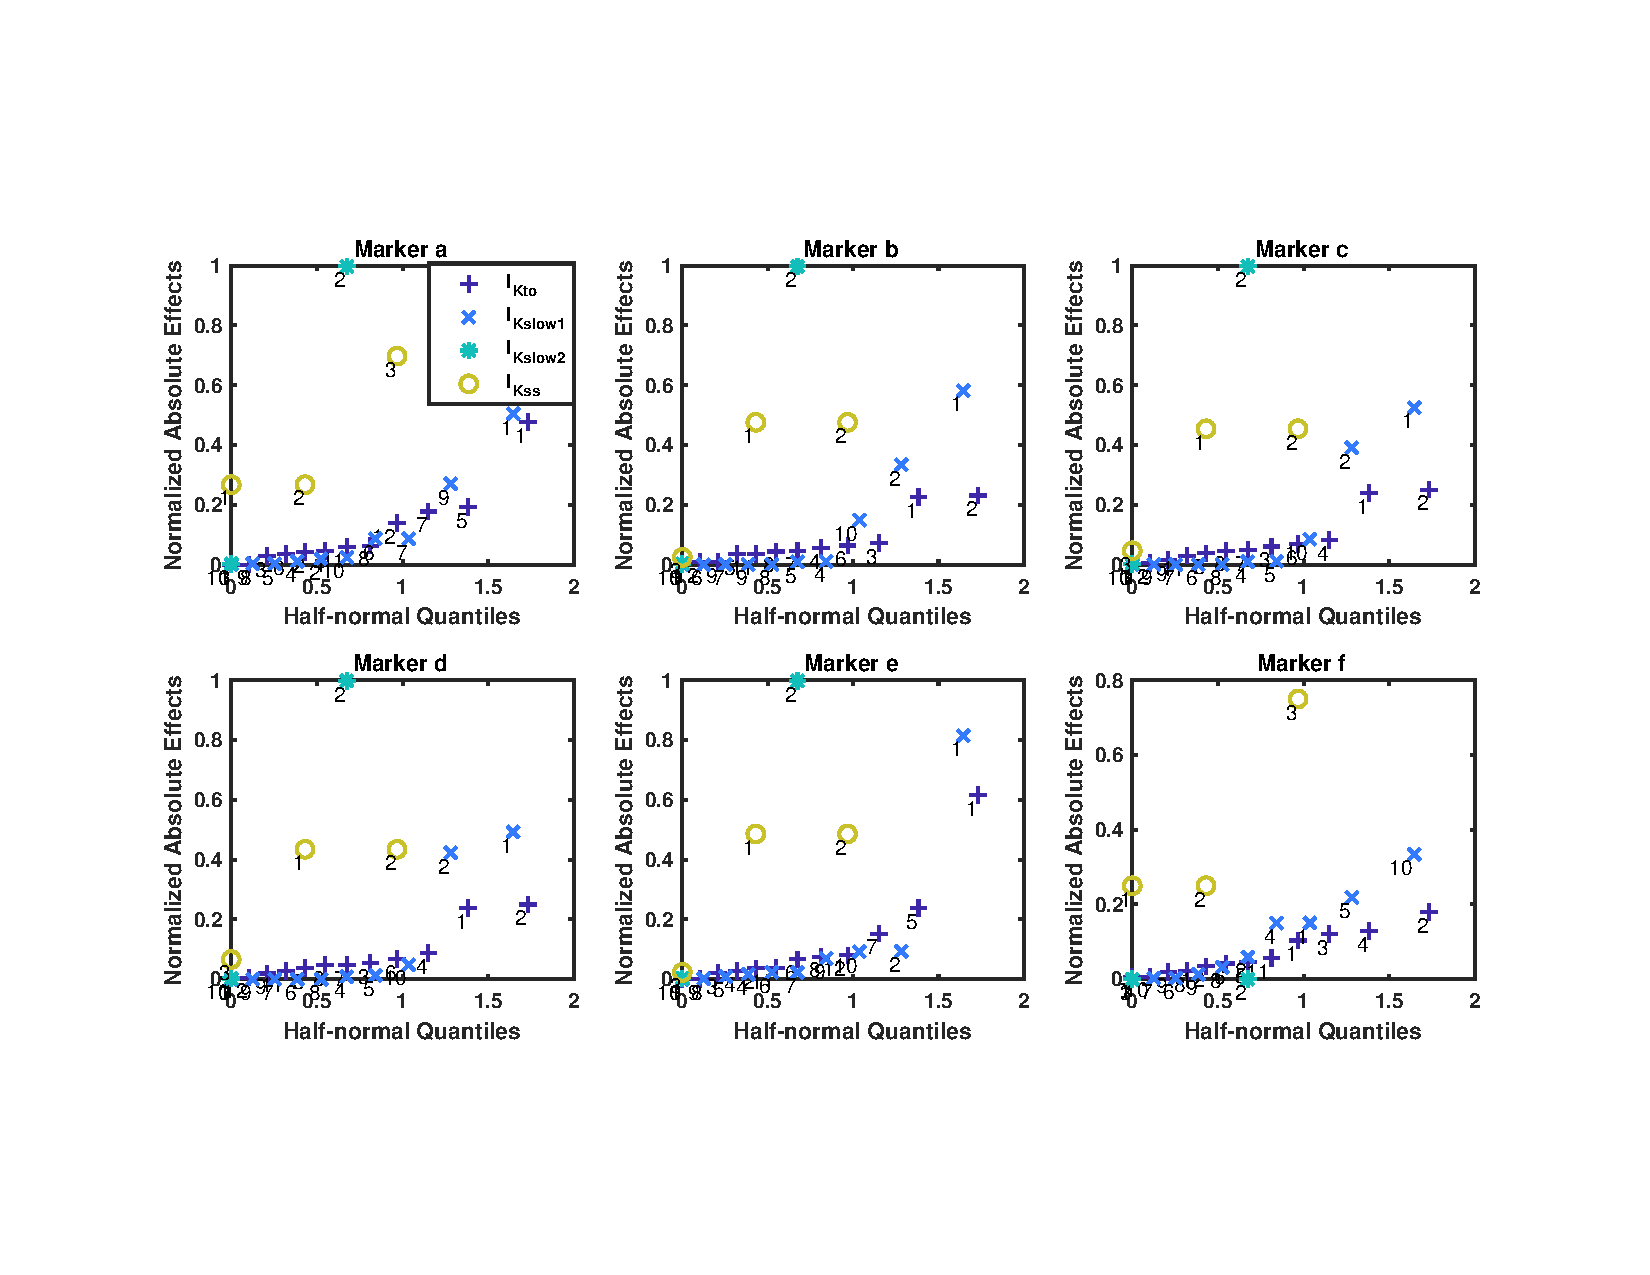
\includegraphics{figs/half-norm.pdf}
    \caption{Half-normal plots of factorial effects for identifying significant parameters in the four current models on (a) Marker a, (b) Marker b, (c) Marker c, (d) Marker d, (e) Marker e, and (d) Marker d.}
    \label{fig:half-norm}
\end{figure}

Figure~\ref{fig:calib_param} shows the selected parameters, highlighted in different colors according to their functional roles in channel kinetics. We categorized the calibration parameters into four classes: The red represents the voltage-threshold parameters and the green voltage slopes, controlling the voltage dependence, the blue scale factors of kinetic functions, and purple time-constant shifters. Note that the voltage-dependence parameters in red and green appear multiple times across different equations. This parsimonious model design is intended to maximize the structural regularization to minimize overfitting. In general, voltage-threshold and time-constant-shifting parameters impact the current traces more than others. 
\begin{figure}[!ht]
    \centering
    \includegraphics{figs/calib_param.pdf}
    \caption{Selected parameters by the sensitivity analysis of (a) I\textsubscript{Kto}, (b) I\textsubscript{Kslow1}, (c) I\textsubscript{Kslow2}, and I\textsubscript{Kss}. Parameters are highlighted in different colors according to their functional roles in channel kinetics.}
    \label{fig:calib_param}
\end{figure}

\subsection{Model Fitness}
We tested various nonlinear optimization algorithms in the proposed model calibration routine that support box constraints, and the BFGS algorithm provided the most reliable results. A separate accuracy metric is used to measure the goodness-of-fit and potential prediction power of the calibration results rather than reporting the final objective function value. The objective function (i.e., sum of RMSEs) does not provide a straightforward interpretation that makes it difficult to evaluate the calibration performance. $R^{2}$, defined in \eqref{eq:r2}, is the most common prediction accuracy metric ranging from 0 to 1 for linear regression models that represents the proportion of variation in data that is explained by the model. However, this interpretation is not applicable to nonlinear models because the variance decomposition in \eqref{eq:var_decomp} does not hold anymore.
\begin{align}
    \label{eq:r2}
    &R^{2} = 1 - \frac{\sum_{i=1}^{n}(y_{i}-\hat{y_{i}})^2}{\sum_{i=1}^{n}(y_{i}-\bar{y})^2} \\
    \label{eq:var_decomp}
    &\sum_{i=1}^{n}(y_{i}-\bar{y})^2 = \sum_{i=1}^{n}(\hat{y_{i}}-\bar{y})^2+\sum_{i=1}^{n}(y_{i}-\hat{y_{i}})^2
\end{align}

Therefore, a pseudo-R-squared measure, proposed in \citep{li2019prediction} is used to evaluate the model fitness in this study. This nonlinear $R^{2}$ measure is based on the concept of linear correction of prediction function, allowing the variance decomposition for nonlinear functions, which guarantees straightforward interpretation and normalized scores between 0 and 1 as in the classical $R^{2}$. Figure~\ref{fig:model_fitness}(a) and (c) present averages of nonlinear $R^{2}$ values over voltage steps from -30 to 50 mV by 10 mV step size for WT and MGAT1KO, respectively. In most cases, more than 90 \% of variances on average are explained by models (WT: $0.9624 \pm 0.0051$; MGAT1KO: $0.8938 \pm 0.0077$). The model fitness measures in MGAT1KO are lower than WT in general. It is expected that the small current magnitude of MGAT1KO challenges the calibration process. We randomly select a cell from each group and compare the actual model predictions and experimental I\textsubscript{Ksum} traces in Figure~\ref{fig:model_fitness}(b) and (d) to validate the model calibration results further. As shown in Figure~\ref{fig:model_fitness}(d), MGAT1KO at -30 mV clamp voltage, small and noisy current trace, results in decreased $R^{2}$, 0.8335. The fitting was performed on \DIFaddbegin \DIFadd{Intel }\DIFaddend 4-core Xeon E7-4830 processors. Without parallel computing on multiple cores, each cell took an average of $438.1 \pm 6.8$ \DIFaddbegin \DIFadd{s }\DIFaddend to complete the data assimilation procedure for 5 random initial points. It took an average of $333.8 \pm 6.0$ s with multicore processing, which is ~31 \% \DIFdelbegin \DIFdel{efficient}\DIFdelend \DIFaddbegin \DIFadd{efficiexnt}\DIFaddend .
\begin{figure}[!ht]
    \centering
    \includegraphics{figs/model_fitness.pdf}
    \caption{Bar graphs of the averages of nonlinear $R^{2}$s for nine voltage steps from -30 mV to 50 mV by the 10 mV step size for (a) WT and (c) MGAT1KO. Exemplary actual fitness between model predictions (in green) and experimental I\textsubscript{Ksum} recordings (in pink) at six voltage steps of (b) cell 6 in WT and (d) cell 12 in MGAT1KO.}
    \label{fig:model_fitness}
\end{figure}

\subsection{Prediction of K\textsubscript{v} Activities}
The in-silico modeling predicts that chronic reduction in cardiomyocyte N-glycosylation results in significant changes in channel steady states and kinetic behaviors. The most notable result in the in-vitro experimental data was the significant reduction in the current density in response to a 50-mV test potential. To verify this observation, Figure~\ref{fig:current_density} presents the prediction results of the current-density relationship of the four K\textsuperscript{+} currents. The model predicts the compatible result showing the I\textsubscript{Kto}, I\textsubscript{Kslow1}, and I\textsubscript{Kslow2} densities are significantly reduced in MGAT1KO cardiomyocytes, while there are no remarkable differences in I\textsubscript{Kss}. Note that in the in-vitro experiments, bi-exponential fitting was used, in which the two delayed rectifier currents are combined (I\textsubscript{Kslow}), because it is difficult to reliably fit a tri-exponential function with a relatively short voltage step (4.5 s here) \citep{liu2011dissection}. In contrast, although the proposed model-guided data assimilation distinguishes K\textsubscript{v}1.5 and K\textsubscript{v}2.1, it shows compatible prediction results with the experimental data as well as high fitness accuracy ($\sim$90 \% $R^{2}$) \citep{ednie2019reduced}.
\begin{figure}[!ht]
    \centering
    \includegraphics{figs/current_density.pdf}
    \caption{Current-density relationships of the major K\textsubscript{+} currents: (a) I\textsubscript{Kto} (b) I\textsubscript{Kslow1}, I\textsubscript{Kslow2}, and I\textsubscript{Kss}.}
    \label{fig:current_density}
\end{figure}

Another aberrant activity of K\textsuperscript{+} currents was slower inactivation of the delayed rectifier currents in MGAT1KO cardiomyocytes. Figure~\ref{fig:time_constants} shows the prediction results of the inactivation time constants of I\textsubscript{Kslow1} and I\textsubscript{Kslow2}. The computer models successfully capture this trend, resulting in the time constant of inactivation in for I\textsubscript{Kslow1} ($\tau_{i}^{(\mathrm{Kslow1})}$) being estimated to be significantly slowed in MGAT1KO compared to WT, i.e., $\sim$348.9 ms, as shown in Figure~\ref{fig:time_constants} (a). I\textsubscript{Kslow2} is also slowed (see Figure~\ref{fig:time_constants} (b)). The inactivation time constants are important because they determine how slowly I\textsubscript{Kslow1} and I\textsubscript{Kslow2} inactivate and, in turn, affect the repolarization of the AP significantly. $\tau_{i}^{(Kslow1)}$ show higher variability than other currents to address most of the decaying portion of I\textsubscript{Ksum}. This is likely due to the fact that while K\textsubscript{v}4.2 and K\textsubscript{v}2.1 are O-glycosylated, K\textsubscript{v}1.5 possess a single occupied N-linked glycosylation. Hence, I\textsubscript{Kslow1} is more affected by reduced N-glycosylation. A plot is not provided here, but there is no significant effect on I\textsubscript{Kto} for membrane potential greater than 0 mV. It is worth mentioning that the proposed method was able to extrapolate $\tau_{i}^{(\mathrm{Kslow2})}$ that is greater than 5 s from the 4.5-s-pulse protocol, which shows the generalization power of the in-silico modeling.
\begin{figure}[!ht]
    \centering
    \includegraphics{figs/time_constants.pdf}
    \caption{Inactivation time constants of (a) I\textsubscript{Kslow1}, and (b) I\textsubscript{Kslow2}.}
    \label{fig:time_constants}
\end{figure}

\subsection{Cellular Variability}
The calibrated parameters are in a 61×20 matrix (i.e., 31 observations in WT and 30 in MGAT1KO, and there are 20 calibration parameters), and we apply t-SNE to encapsulate this high-dimensional data into three-dimensional space to visualize each data point. Figure~\ref{fig:embd_result} (a) presents the visualization of the t-SNE embedding of the calibration results. It shows not only clear differences between the two groups but also variances of cells (i.e., data points) within the groups across the entire data, indicating that MGAT1KO cells have higher variance in the aggregated kinetic parameter space. Determinants of the covariance matrices of the 3D embedding data to quantify the variability of WT and MGAT1KO in the kinetic parameter space. It turns out that WT has 38 \% higher variability than MGAT1KO. 

To further investigate it, we generated the histograms of the maximum conductance of I\textsubscript{Kslow1} (\textit{G}\textsubscript{Kslow1}), which is the most significant parameter determining the magnitude of the current (see Figure~\ref{fig:embd_result} (b)), and experimental I\textsubscript{K} density from the in-vitro data. There is clear skewness in MGAT1KO I\textsubscript{Ksum} density (small variance), while WT I\textsubscript{K} density is more disperse (high variance). Calibrated parameters, for example \textit{G}\textsubscript{Kslow1}, likely show smaller variations in MGAT1KO to address this trend in the experimental data. It is likely due to significant I\textsubscript{K} reduction in the diseased group combined with the elimination of complex N-glycosylation, thereby minimizing potential variability of N-glycan structures
\begin{figure}[!ht]
    \centering
    \includegraphics{figs/embd_result.pdf}
    \caption{(a) Low-dimensional embedding of calibration parameters into 3D space. Blue circles - WT myocytes ($n=31$); Red triangles - MGAT1KO myocytes ($n=30$). (b) Histogram of the calibrated kinetic parameter for maximum conductance of I\textsubscript{Kslow1} (\textit{G}\textsubscript{Kslow1}), which is the most significant factor determining the magnitude of I\textsubscript{Kslow1}. (c) Histogram of experimental I\textsubscript{Ksum} density.}
    \label{fig:embd_result}
\end{figure}

\section{Discussion and Conclusions}
Repolarization is a complex process that involves various K\textsubscript{v} isoforms. It is critical to understand the unique properties and functional roles of each K\textsubscript{v} to investigate pathological mechanisms of diseased cardiomyocytes that contribute to fatal heart diseases. However, current laboratory techniques, such as whole-cell patch-clamp recording, are not able to measure individual activities of K\textsubscript{v} isoforms reliably that activate, inactivate, and close at overlapping times during recordings, except through the attempt to remove K\textsubscript{v} isoform activity through less-than-fully-specific pharmacological intervention. Thus, only the sum of the different K\textsubscript{v} isoform activities can be measured as a single current trace, I\textsubscript{Ksum}. Hence, it is necessary to decompose I\textsubscript{Ksum} into individual K\textsuperscript{+} currents and estimate their channel activity via data assimilation. This paper presents a subject-specific concurrent data assimilation method for learning K\textsubscript{v} activities using multiple I\textsubscript{Ksum} recordings simultaneously for each cell. A case study is provided using our in-vitro experimental data of mouse cardiomyocyte I\textsubscript{K} in control conditions (WT) and under conditions of reduced complex N-glycosylation (MGAT1KO). We evaluate the calibration results using an adjusted $R^2$ measure for nonlinear models that preserves the interpretability of the classical $R^2$ based on the variance decomposition for linear models. Experimental results show the proposed method explains more than 90\% of variances by calibrated models in most cases (WT: $0.9624 \pm 0.0051$; MGAT1KO: $0.8938 \pm 0.0077$). 
\DIFaddbegin 

\DIFadd{In addition to achieving a high degree of goodness-of-fit, it is important to determine the source of uncertainty and variability in model predictions to build trustworthy models. Until recently, the conventional approach to developing cardiac models and fitting model parameters has involved using single values. As a result, most mathematical models currently in use only provide point estimates without quantifying uncertainty \mbox{%DIFAUXCMD
\citep{johnstone2016uncertainty}}\hskip0pt%DIFAUXCMD
. Although variances across cells are provided in the model predictions of current density and inactivation times in Figure~\ref{fig:current_density} and Figure~\ref{fig:time_constants}, it remains elusive whether the variability arises from model uncertainty or true cellular variability in the data. Statistical methods for uncertainty quantification (UQ) in cardiac models, such as Bayesian inferences or Gaussian process emulators, have been proposed \mbox{%DIFAUXCMD
\citep{johnstone2016uncertainty,coveney2020sensitivity}}\hskip0pt%DIFAUXCMD
. Exploring the incorporation of UQ techniques into data assimilation is a topic for future research. }\DIFaddend A GUI application is provided \DIFdelbegin \DIFdel{to make }\DIFdelend \DIFaddbegin \DIFadd{as }\DIFaddend an enabling tool for biomedical scientists without full expertise in modeling and computational analysis.

The estimation of kinetics provides novel insights into potential mechanisms by which specific K\textsubscript{v} isoforms contribute to the overall reduction in I\textsubscript{K} observed in in-vitro experiments following chronic reductions in N-glycosylation. Thanks to the cell-specific approach, prediction uncertainty is quantified, and error bars are provided in the prediction results. Further, calibrated parameters are visualized via low-dimensional embedding that allows for encapsulating calibrated parameters in 3D space and, in turn, visualizing the variability across cells. WT cells show higher variability than MGAT1KO myocytes, which is likely due to significant I\textsubscript{K} reduction in the diseased group, combined with the elimination of complex N-glycosylation, thereby minimizing potential variability of N-glycan structures. The proposed method and pertinent software show strong potential for studying K\textsubscript{v} kinetics in various heart diseases. However, there are still some limitations and challenges that need to be addresses in future work. One of the main limitations of this study is that it does not address the interactions of K\textsubscript{v} with other major VGICs, namely Na\textsubscript{v} and Ca\textsubscript{v}, and cellular-level processes. Thus, causal inference of the effects of chronic glycosylation deficiency is limited. We plan to develop an integrative modeling method for learning activities of major VGICs together.  

\section*{Funding}
This work is supported by the National Science Foundation (MCB-1856132 to HY and HK), (MCB-1856199 to EB and AE), (IOS-1146882 and IOS-1660926 to EB), and the American Heart Association (Postdoctoral Fellowship 15POST25710010 to AE). HY and HK would also like to thank the NSF I/UCRC Center for Health Organization Transformation (CHOT) award NSF IIP-1624727 for the support of their research work. Any opinions, findings, or conclusions found in this research are those of the authors and do not necessarily reflect the views of the sponsors. 

\section*{Disclosure of Interest}
The authors report there are no competing interests to declare.

\section*{Consent and Approval}
This research does not involve any human participants or data. Therefore, no consent or approval was required for this study.

\bibliographystyle{chicago}
\spacingset{1}
\bibliography{Bibliography}

\end{document}
